\documentclass[tikz]{standalone}

\usepackage[greek,english]{babel}

\usepackage{pgfplots}
\usetikzlibrary{decorations.pathreplacing}

\pagecolor{white}

\begin{document}
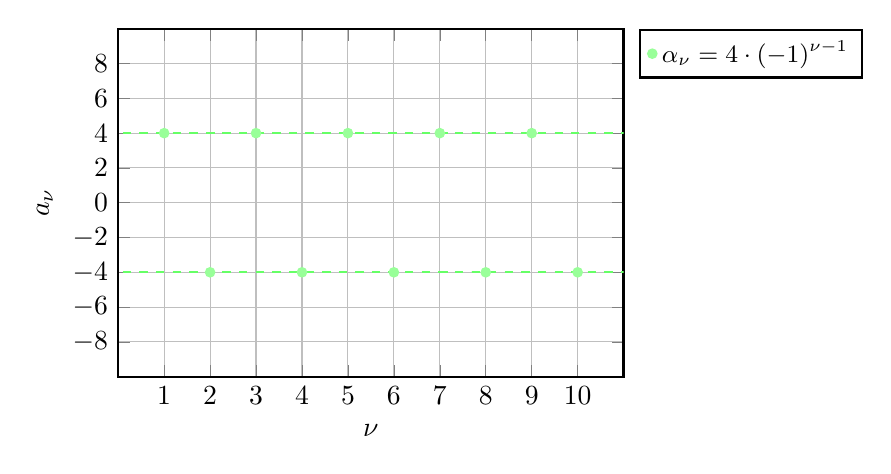
\begin{tikzpicture}
\begin{axis}[
    width=8cm,
    height=6cm,
    domain=-15:15, 
    xmin=0,
    xmax=11,
    ymin=-10,
    ymax=10,
    thick,
    ytick={-8,-6,-4,-2,0,2,4,6,8},
    xtick=data,
    legend pos=outer north east,
    mark size=1.5pt,
    xlabel={$\nu$},
    ylabel={$a_\nu$},
    legend cell align={left},
    grid]


\addplot[only marks, green!40!white] coordinates {
(1, 4)
(2, -4)
(3, 4)
(4, -4)
(5, 4)
(6, -4)
(7, 4)
(8, -4)
(9, 4)
(10, -4)
};
\addlegendentry{\small $\alpha_\nu = 4 \cdot (-1)^{\nu - 1}$ }

\addplot[red, domain=0.1:11,restrict y to domain=0:10, samples=100, green!60!white,forget plot,dashed]  {4};
\addplot[red, domain=0.1:11,restrict y to domain=-10:10, samples=100, green!60!white,forget plot,dashed]  {-4};


\end{axis}
\end{tikzpicture}
\end{document}
